\section{Abstract}

A global contrast between oceanic and continental lightning very low frequency energy is observed using the World Wide Lightning Location Network (WWLLN).
Strokes over the ocean are found to be stronger on average than those over land with a sharp boundary along a majority of coastlines.
A linear regression method is developed to account for the spatial and temporal variation of WWLLN in order to perform a multi-year and global analysis of stroke energy distributions.

The results are corroborated with data from the Lightning Imaging Sensor, the Optical Transient Detector, and the Earth Networks Total Lightning Network.
These systematic comparisons lead to the conclusion that there exists a strong difference in the energetics between land and ocean thunderstorms that results in a higher fraction of more powerful strokes over the oceans. 


\section{Introduction}

Global surveys of lightning climatology have routinely shown more lightning activity over continents than over oceans \citep{Christian2003}.
The difference in activity is often attributed to changes in the convective regimes in the clouds.
\citet{Williams2002} and \citet{Williams2005} discuss aerosol concentration, wet bulb temperature, and cloud base height as dominant mechanisms of the difference in cloud electrification.
\citet{Zipser1994} suggests updraft velocity due to differential surface heating may lead to the difference in observed flash rates.
\citet{Boccippio2000} shows the total flash counts may be due to a lesser frequency of occurrence of oceanic storms and not a difference in the storms themselves.

Along with the difference in flash rates, there have been several observations suggesting an inherent difference in the lightning peak currents and optical radiance between land and ocean storms \citep{Seity2001, Ishii2010}. 
The U.S. National Lightning Detection Network (NLDN) observed higher average peak currents for negative cloud to ground (CG) strokes off of the coast, but the NLDN is limited in range for oceanic strokes near to coastlines \citep{Rudlosky2010, Lyons1998}.
\citet{Boccippio2000} observed with LIS/OTD an increase in the optical radiance and extent of oceanic flashes compared to those over land.
It was suggested that either a more energetic lightning generation process or a reduced cloud optical depth for the oceanic storms could produce the increased optical radiance.
However, it could not be be determined whether the more radiant flashes were caused by changes in the flashes or in the cloud optical depth using just the available satellite data.

As of January 2013, the World Wide Lightning Location Network (WWLLN, see wwlln.net) consists of 70 very low frequency (VLF) stations around the world allowing it to detect with a 5~km location and $15\mu$s timing accuracy and an estimated overall stroke detection efficiency of 11\% \citep{Hutchins2012a, Abarca2010,Rodger2009}.
An upgrade to the WWLLN allows for the network to measure radiated VLF stroke energies in addition to stroke locations \citep{Hutchins2012}.
The capability to measure stroke energies as well as the global coverage of the network allows for a global comparison of stroke energies over land and ocean regimes.

A comparison is made between the global stroke count climatologies of WWLLN and the 13-year Lightning Imaging Sensor (LIS) and 5-year Optical Transient Detector (OTD) flash count climatologies. 
The LIS (1997-present) and OTD (1995-2000) are nearly identical satellite-based lightning detectors flown in low earth orbit that observe total lightning activity from individual thunderstorms for 90 sec and 2 min, respectively, as the satellite passes overhead.
The LIS observes storms from an inclined orbit of 35$^\circ$ at an altitude of 402 km while the OTD observed storms from an inclined orbit of 70$^\circ$ at an altitude of 740 km \citep{Christian1999, Christian2003}.
Since WWLLN preferentially detects high-energy strokes \citep{Hutchins2012a} a direct comparison between the two systems, as described in \citet{Virts2013}, gives a comparison between high and low-energy strokes because of the detection biases of the two systems.

A second ground based detection network, the Earth Networks Total Lightning Network (ENTLN), is used to corroborate the results of the WWLLN data.
ENTLN is a higher density, broadband (1~Hz to 12~MHz receiver) network with about 500 operational stations in the United States \citep{Heckman2010}.
The network utilizes a time of arrival method to determine the location of each stroke, where a minimum of 8 stations is required to produce a valid solution.
From the recorded waveforms ENTLN infers polarity, peak current, and stroke type \citep{Liu2011a}.

\section{Linear Regression Analysis}
\label{secLinReg}

In order to compare WWLLN energy data over large spatial and temporal scales the data needs to be processed to account for the regional variations in detection efficiency and temporal changes in network performance.
To examine the spatial changes in stroke energy while accounting for network variability a linear regression method is developed.

Energy data for each day is binned every 0.5$^\circ$ in latitude and longitude.
The strokes in each bin are split into 10 energy deciles each containing $J$ strokes, with the mean energy of each decile, $i$, given by:

\begin{equation}
\overline{E_i} = \frac{\sum_{j=1}^J E_{i,j}}{J} 
\end{equation}

$\overline{E_i}$ has a power law dependence on decile number due to the lognormal distribution of stroke energies.
In order to make a linear regression between $\overline{E_i}$ and decile number $i$, the log$_{10}$ of $\overline{E_i}$ is used. 
A linear regression is found between $\text{log}_{10}(\bar{E_i})$ and $i$ to get an approximation of the mean energy with decile:

\begin{equation}
\text{log}_{10}(\overline{E(i)}) = C + \frac{\partial \text{log}_{10}(\overline{E_i})}{\partial i} i
\end{equation}

The first parameter from the fit, $C$, corresponds to the overall mean of the stroke energies in the particular spatial bin.
It is not used in this analysis since $C$ greatly depends on the network coverage at the time and location where it calculated.
$C$ will be larger where coverage is lower (WWLLN detecting only strong strokes) and lower with high coverage (WWLLN detecting both strong and weak strokes).
By using the regression method the network coverage and variable detection efficiency is factored out of the energy distribution into $C$ allowing for the shape of the energy distribution to be examined directly.

The second parameter, $\frac{\partial \text{log}_{10}(\overline{E_i})}{\partial i}$, is the slope of the regression and will be used to study the energy changes between land and ocean regimes.
$\frac{\partial \text{log}_{10}(\overline{E_i})}{\partial i}$ is the measure of how much (logarithmically) the average stroke energy changes from one decile to the next.
So a value of $\frac{\partial \text{log}_{10}(\overline{E_i})}{\partial i}$~=~0.1 at a location will increase the mean stroke energy by $10^{0.1}~=~25\%$ per decile, while a value of 0.2 will increase by $10^{0.2} = 58\%$ per decile.
The regression slope will be higher for either more high-energy strokes or fewer low-energy strokes.
The low-energy tail of the energy distribution is mostly set by the efficiency of the network, while the high end is always well detected even where the network is thin.
As $C$ captures the effects of the network performance, the slope of the regression will be mainly set by the energy of the strokes in the high-energy tail of the distribution.

An example of the linear regression method is shown in Figure~\ref{linRegTheory} using 15~days of data from 1-15 June 2012, separated into land (black) and ocean (gray) strokes.
The stroke counts are split into the ten decile bins outlined in Figure~\ref{linRegTheory}a.
$\overline{E_i}$ is shown in Figure~\ref{linRegTheory}b with the corresponding regressions plotted on top of the points.
Departures from the regression are acceptable as only the trend of increasing energy is important and not an exact fit.

\begin{figure}[ht!]
   \centering
   \noindent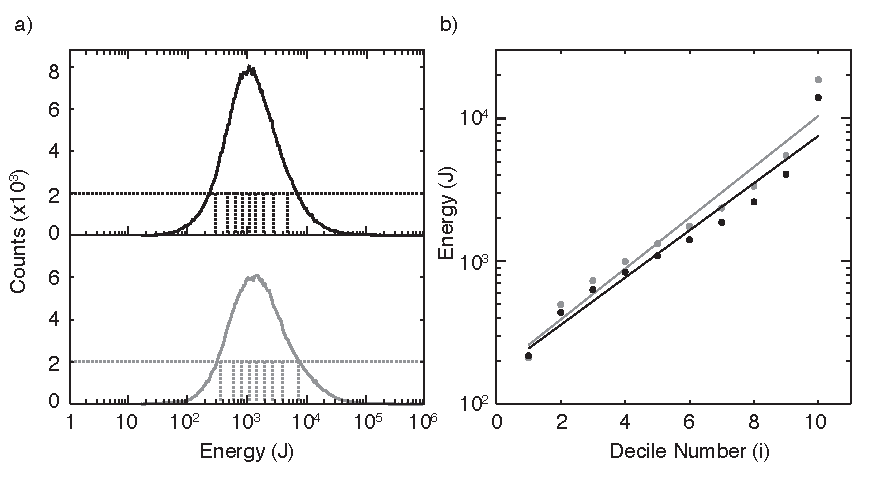
\includegraphics[width=20pc]{LandSea/Figures/1_linearRegression.pdf} 
   \caption{WWLLN data from 1-15 June 2012 for global strokes grouped into land (black) and ocean (gray) to demonstrate the linear regression method. a) Shows two energy distributions with the corresponding energy decile bins (dashed lines). b) is the plot of mean energy $\overline{E_i}$ in each bin with the linear regression (solid lines).}
   \label{linRegTheory}
\end{figure}

\section{Regression Slope Maps}

This technique is applied over 3 years of WWLLN data from May 2009 through May 2012 on a 0.5$^\circ$ grid, with the resulting regression slopes shown in Figure~\ref{regMap}.
For this analysis the calculated regressions must have an R-square value of at least 0.80 to be used.
In general higher slopes are seen over oceans and lower slopes over land, except for several regions of low detection efficiency (e.g. off the shore of Madagascar) and regions such as the Andes mountain range.
The map is similar to Figure~\ref{virts}, adapted from \citet{Virts2013}, which shows the ratio of the WWLLN normalized stroke climatology to the LIS/OTD normalized flash climatology.
The climatologies are normalized by their total stroke and flash counts respectively.
Figure~\ref{virts} is the spatial distribution of where WWLLN preferentially detects more strokes than LIS/OTD due to the bias of WWLLN towards detecting the most energetic strokes.
Comparing the stroke and flash data directly is possible as a majority of flashes have only the first, and strongest, stroke detected by WWLLN \citep{Abarca2010}.


\begin{figure}[ht!]
   \centering
   \noindent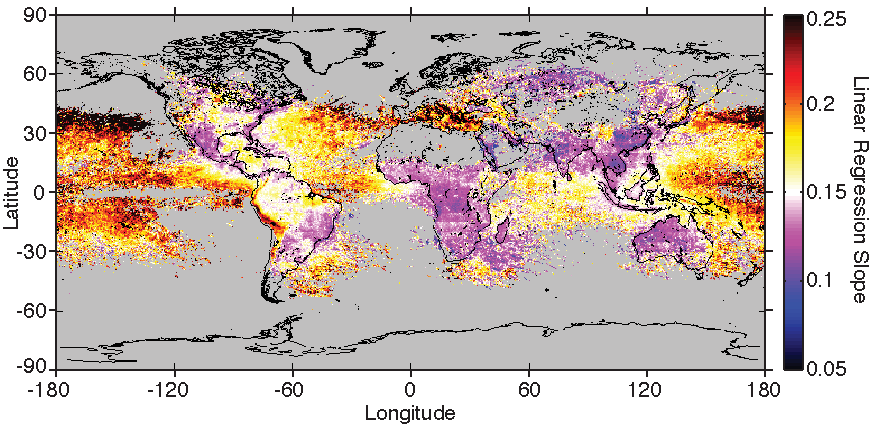
\includegraphics[width=20pc]{LandSea/Figures/2_regMap.pdf} 
   \caption{Slope of the linear regression used on the energy distribution as described in the text. High slope corresponds to a larger high-energy tail in the energy distribution as there are relatively more high-energy strokes.}
   \label{regMap}
\end{figure}

\begin{figure}[ht!]
   \centering
   \noindent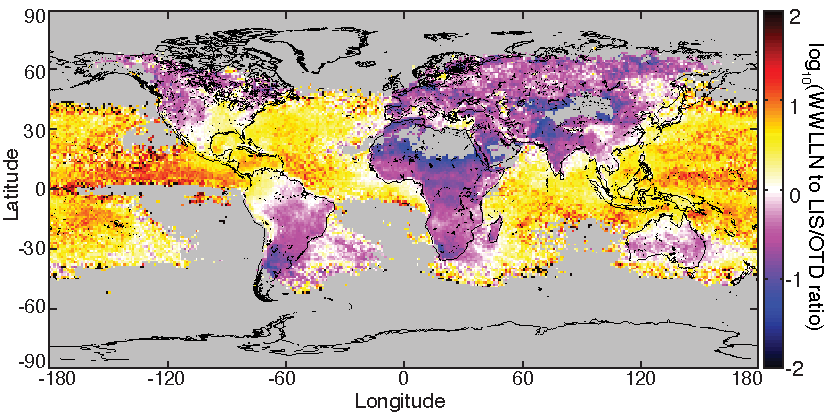
\includegraphics[width=20pc]{LandSea/Figures/3_lisMap.pdf} 
   \caption{Ratio of the WWLLN stroke count density climatology to the LIS/OTD flash count density climatology normalized by their relative total counts, adapted from \citet{Virts2013}.}
   \label{virts}
\end{figure}

The same linear regression was applied to the 2011 ENTLN data for a region over North America.
The absolute peak current was used for the regression instead of the stroke energy with the results in Figure~\ref{regMapENTLN}.
The land-ocean contrast is seen strongly in the ENTLN dataset, particularly over Mexico, Cuba and Haiti.
The difference also exists off the coast of the southeastern United States, but the contrast is not as strong (slope increase on the order of 0.01 instead of 0.1).

\begin{figure}[ht!]
   \centering
   \noindent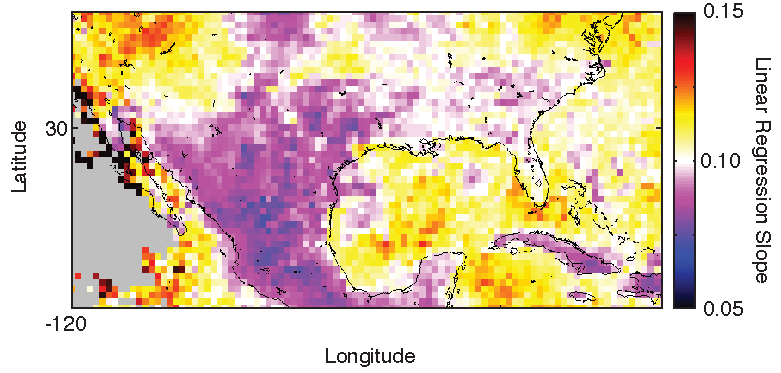
\includegraphics[width=20pc]{LandSea/Figures/4_regMapENTLN.pdf} 
   \caption{Slope of the linear regression used on the 2011 ENTLN absolute peak current distribution as described in the text. High slope corresponds to a larger high peak current tail in the distribution.}
   \label{regMapENTLN}
\end{figure}

For the ENTLN data the linear regression slopes only range from 0.05 to 0.15 compared to 0.05 to 0.25 for the WWLLN regressions.
Since energy is related to peak current by $E_{stroke} = 2229 \times | I_{peak} | ^{1.62}$ \citep{Hutchins2012}, $\text{log$_{10}$}(\overline{E_i})$ will be 1.62 times higher than $\text{log$_{10}$}(\overline{I_{peak,i}})$.
The range of the slopes for the ENTLN regression should then be correspondingly lower by a factor of 1.62, or from 0.03 to 0.15.

\section{Stroke Distributions}

The global ratio of the land and ocean stroke distributions clearly shows the prevalence of higher energy strokes over oceans.
The energy distribution of the WWLLN data is found for the set of strokes occurring over land and for the strokes occurring over oceans.
The ratio of these ocean and land energy distributions is shown in Figure~\ref{ratioComp}.

\begin{figure}[ht!]
   \centering
   \noindent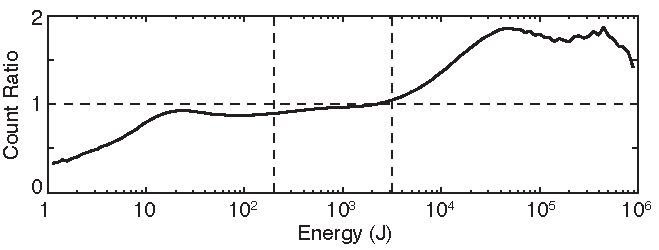
\includegraphics[width=20pc]{LandSea/Figures/5_distribution.pdf} 
   \caption{The ratio of ocean to land counts for WWLLN within each energy bin. The dashed horizontal line is a ratio of 1. The vertical dashed black lines in show the 15th and 85th percentile levels for the distribution.}
   \label{ratioComp}
\end{figure}

The ocean-land ratio starts increasing quickly with increasing energy at 3000~J, showing there are relatively more high-energy (top 15\% of stroke energy) strokes over the oceans than over land.
Similarly there is a general decrease in the ratio for decreasing strokes energies, with the downward trend interrupted with a small bump near 10~J.

\section{Regional Contrast}

In Figures~\ref{regMap} and~\ref{virts} there is an evident overall difference between land and ocean strokes, and it can be seen to vary sharply across most coastlines.
This raises the question of whether network detection efficiency across the coastline should be considered as a potential cause for the change.
Three regions are chosen for closer examination, shown outlined by the white boxes on top of a map of the WWLLN relative detection efficiency in Figure~\ref{wwlln_regional}a: North America, Western Africa, and Northeastern Brazil. 

\begin{figure}[ht!]
   \centering
   \noindent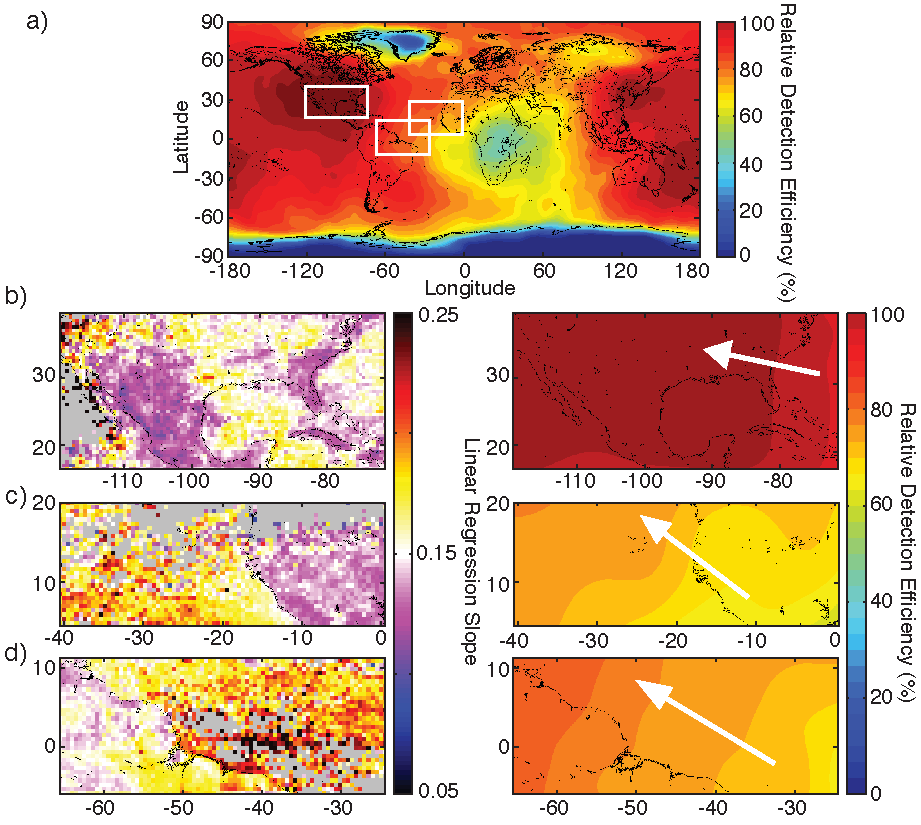
\includegraphics[width=20pc]{LandSea/Figures/6_wwlln_regional.pdf} 
   \caption{Regional maps of the linear regression slopes in the left column with respective WWLLN relative detection efficiency maps on the right. Selected regions outlined in a) on top of the map of the May 2009 through May 2012 average relative detection efficiency. b) shows the Continental United States and Gulf of Mexico, c) Western Africa, and d) Northeast Brazil. The white arrows point in the direction of increasing relative detection efficiency.}
   \label{wwlln_regional}
\end{figure}

WWLLN has an inherent bias towards more readily detecting low energy strokes over oceans than over land.
This is due to lower VLF wave attenuation over oceans, so low-energy strokes propagating over the ocean can reach more WWLLN stations compared to the same stroke traveling over land.
Hence WWLLN is naturally biased to predominately detect only the highest strokes over land, and relatively more lower energy strokes over water \citep{Hutchins2012}.
The method of linear regression described in Section~\ref{secLinReg} should remove most of this bias in WWLLN, and this can be checked in part by the recent work on relative detection efficiency \citep{Hutchins2012a}.
The three regions chosen in Figure~\ref{wwlln_regional} were chosen such that the gradient of relative detection efficiency is changing parallel to the coastline.

Over North America and the Gulf of Mexico, Figure~\ref{wwlln_regional}b, the strokes over Mexico, Florida, Cuba, and Haiti are all weaker than those over the nearby ocean.
This is also seen with the ENTLN in Figure~\ref{regMapENTLN}.
The relative detection efficiency (see \citet{Hutchins2012a}) is fairly uniform over this region with the largest change occurring over the Atlantic where there is no change to the regression slope.
Over the central United States there is a large region of high stroke energies, this is also observed in the ENTLN regression slope (Figure~\ref{regMapENTLN}) and LIS/OTD count ratio (Figure~\ref{virts}) data. 

In Western Africa, Figure~\ref{wwlln_regional}c, there is a clear difference between the land and the ocean.
The coast shows a very sharp change in the stroke strength.
The changing detection efficiency in this case is parallel to the coast and would not affect the variation in stroke energy at the coastline.

The difference in Brazil, shown in Figure~\ref{wwlln_regional}d, is similar to that over Western Africa with the exception of the increased stroke energies seen over Amazon River delta.
Even with the increase over the delta there is still a contrast off of the coast with the change in regression slope comparable to the coastline northwest of the delta.

\section{Conclusion}

A linear regression method is developed and applied to the WWLLN dataset in order to examine global and regional changes of lightning stroke strength over several years of network data.
Through comparing WWLLN, ENTLN, and LIS/OTD the difference between stroke strength is seen to be highly dependent on whether the storms occur over land or over ocean with a sharp boundary occurring along most coastlines.
Smaller regions are examined to show that the contrast along coastlines is not due to abrupt changes in the detection efficiency of the networks.
The sharpness of the coastal changes, less than 100~km, suggests the effect is due to a local phenomena and not be caused by large scale changes in the convective land-ocean regions.
Changes exist within continental regions, but these transition were not examined as the underlying change between regimes is not as sharp as for coastlines.


